\documentclass[12pt,twoside]{article}
\usepackage[english]{babel}
\usepackage[utf8]{inputenc}
\usepackage{algorithm,algpseudocode,amsmath,amssymb,amsfonts,amsthm,array,bm,caption,cases,color,fancybox,fancyhdr,float,fontenc,graphicx,longtable,lipsum,pdfpages,pstricks,subcaption,scalefnt,tikz,times,thmbox,xcolor}
\usepackage[nonumberlist]{glossaries}
\pagestyle{plain}
\usepackage[top=0.5in, bottom=0.5in, left=0.5in, right=0.5in]{geometry}

\begin{document}
\begin{titlepage}

\includegraphics[width=2.5cm]{img/isae.png}
\hspace{60pt}

\includegraphics[width=2.5cm]{img/supaero.jpg}
\hspace{90pt}

\includegraphics[width=3cm]{img/fpms.jpg}
\hspace{50pt}

\includegraphics[width=3cm]{img/umons.eps}
\begin{center}
\vspace{40pt}
{\Large \bf Calibration and Fusion of Stereoscopic and Time-of-Flight Cameras for Zero Gravity Targets Inspection}\\
\vspace{10pt}
by\\
\vspace{10pt}
{\Large Gabriel P. Urbain}\\
\vspace{20pt}
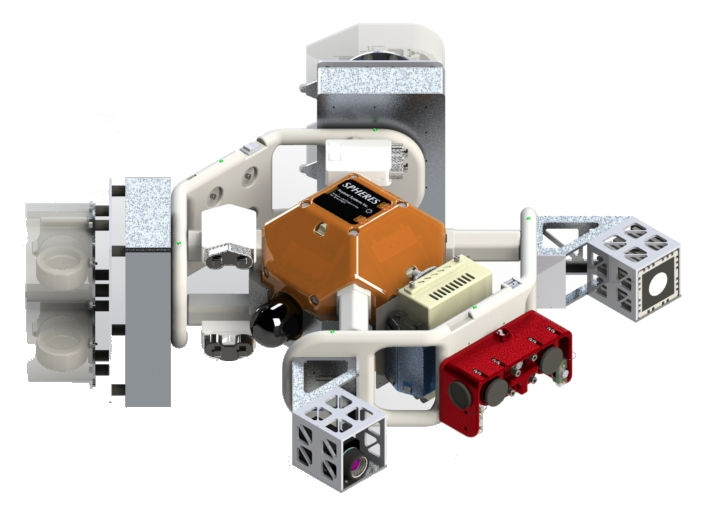
\includegraphics[width=12cm]{img/inspect.png}\\
{\large Submitted to the Department of Electronics, Optronics and Signal Processing, ISAE \\
in partial fulfillment of the \\
requirements for a double degree of \\
\vspace{20pt}
Master of Science in Aerospace Engineering at Supaero, ISAE, France}\\
\vspace{5pt}
and\\
\vspace{5pt}
{\large Master of Science in Electrical Engineering at Facult\'{e} Polytechnique, UMONS, Belgium}\\
\vspace{40pt}
{\Large October 2014}
\end{center}
\hspace{20pt}

\includegraphics[width=4.3cm]{img/mit.eps}
\hspace{320pt}

\includegraphics[width=2cm]{img/ssl.png}
\end{titlepage}


\end{document}